%
% This is the LaTeX file to be used
% for preparation of summaries
% for the Proceedings of the International Congress on Artificial Materials for Novel Wave Phenomena.
%
%
% PROSPECTIVE AUTHORS WISHING TO SUBMIT IN LaTeX
% SHOULD USE AND PROCESS THIS DOCUMENT
%

%%% use for Latex 2.09
%\documentstyle[11pt]{article}

%%% use for Latex 2e
\documentclass[10pt,a4paper]{article}

\usepackage{times}

% Use this if you need to include eps figures:
\usepackage{epsfig,wrapfig}
\usepackage{epstopdf} % for pdflatex

\usepackage{fancyhdr}

\usepackage[lmargin=2.5cm, rmargin=2.5cm,tmargin=3.50cm,bmargin=3.50cm]{geometry}
\usepackage{indentfirst}

\usepackage{titlesec}
\titleformat{\section}[hang]
  {\centering}{\thesection}{1ex}{\normalsize \textsc}%%
\titleformat{\subsection}[hang]
  {}{\thesubsection}{1ex}{\normalsize \textit}%%

\renewcommand\figurename{Fig.}
\renewcommand{\abstractname}{}
\renewcommand{\refname}{\textnormal{\normalsize{\textsc{References}}}}

% In the definition below you may change "acknowledgement" to "acknowledgements"
\newcommand{\acknowledgement}{\section*{\centering{\textnormal{\normalsize{\textsc{Acknowledgement}}}}}}

\renewcommand{\thesection}{ \normalsize \textnormal{\Roman{section}.}}
\renewcommand{\thesubsection}{\normalsize \textnormal{\textsc{\textit{\Alph{subsection}.}}}}

%%%% macros for page setup - please do not change

\pagestyle{fancy}
\fancyhead{} % clear heading
\fancyfoot{} % clear footer
\renewcommand{\headrulewidth}{0.0pt}
\renewcommand{\footrulewidth}{0pt}
\rhead{\footnotesize \textit{12$^{th}$ International Congress on Artificial Materials for Novel Wave Phenomena - Metamaterials 2018} \\
Espoo, Finland, Aug. 27$^{\mathrm{th}}$ - Sept. 1$^{\mathrm{st}}$ 2018}
\lhead{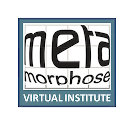
\includegraphics[width=15mm]{MetalogoVI2.eps} \vspace{-0.6cm}}
\chead{}

\parindent=0.4cm


%%% personal macros - start here
%
%
\def\e{\begin{equation}}
\def\f{\end{equation}}
\def\_#1{{\bf #1}}
\def\o{\omega}
\def\E{\varepsilon}
\def\M{\mu}
\def\D{\nabla}
\def\.{\cdot}
\def\x{\times}
\def\Re{{\rm Re\mit}}
\def\Im{{\rm Im\mit}}
\def\l#1{\label{eq:#1}}
\def\r#1{(\ref{eq:#1})}


%
%%% personal macros - end

\begin{document}

%%% Title of paper
\title{\large \textbf{Broadband metamaterial absorber in the X-band.}}
%
%%% Author(s) and affiliation
\def\affil#1{\begin{itemize} \item[] #1 \end{itemize}}
%
\author{\normalsize \bfseries S. umrath$^1$ and \underline{A. Osipov}$^1$
% you will of course remove the next line...
\\ \small (Stefan Umrath, Andrey Osipov, Erich Kemptner)}
%
\date{}
%
\maketitle
\thispagestyle{fancy} % header also to the first page
%
\vspace{-6ex}
\affil{\begin{center}\normalsize $^1$German Aerospace Center (DLR e.V.), Microwaves and Radar Institute, Münchener Strasse 20, 82234, Wessling, Germany
 \end{center}}


%%% Abstract
\begin{abstract}
\noindent \normalsize
\textbf{\textit{Abstract} \ \ -- \ \
%%% Start here with text of abstract
Significant reduction of mono- and bistatic scattering cross
sections of an electrically large metallic cube through the application of
an electrically thin metamaterial low reflection coating operating in the
Ka-band (30--40 GHz) is described. A coating composed of a metallic array
of sub-wavelength sized capacitively loaded strip inclusions printed on top
of a thin, slightly lossy and grounded substrate has been designed and fabricated to experimentally evaluate the performance of the coating in scattering reduction. The scattering reduction is estimated by comparing the
mono- and bistatic scattering patterns of the coated and uncoated cube.
The measurement results are compared with full wave and physical theory
of diffraction simulations, and the possibility of accurately modeling the
low reflection coatings with impedance boundary conditions is pointed out.}
\end{abstract}


\section{Introduction}

The following information is provided to help the prospective contributor preparing papers for submission to the \emph{Twelfth International Congress on Artificial Materials for Novel Wave Phenomena - Metamaterials 2018.}

A contributor should remember that:
\begin{enumerate} \setlength{\itemsep}{-1ex}
\item	The deadline for the paper submission is 4th March 2018; late submissions will not be considered.
\item	Papers should be in English and 3-page long (including figures and references).
\item	Each paper should contain an abstract, a brief conclusion, and a main body where the technical content and novelty of the work are clearly presented.
\item	Authors are requested to thoroughly follow this template when preparing their submission.
\item	Papers should be submitted by uploading a PDF file to the Congress website: \\ http://congress2018.metamorphose-vi.org.
\item	Accepted papers (presented at the conference) submitted in the IEEE-compliant format (i.e., 3-page long, compiled using PDF Xpress and accompanied by the IEEE Electronic Copyright Form) will be published on IEEE Xplore. This will make authors' work available to a much wider audience through indexing services such as ISI Web of Knowledge or Scopus and search engines such as Google. \end{enumerate}

\section{Overview of the Proceedings Format}

All paragraphs, including abstract, figure captions, and references, should be justified at the left and right edges. For the Title use 12-point Times New Roman bold. The font description for the Author List should be 10-point Times New Roman bold, Authors' Affiliation(s) should be 10-point Times New Roman.

\section{Detailed Text Formatting}

Paper size is 21.0 x 29.7-cm (A4). Top and bottom margins are 3.5 cm, and left and right margins are 2.5 cm. Use a single column format.

Each major section begins with a Heading in 10 point Times New Roman centered and numbered using Roman numerals (except for ACKNOWLEDGEMENT and REFERENCES) followed by a period, a single space, and the title using an initial capital letter for each word. The remaining letters are in SMALL CAPITALS.

For the body of your paper, use 10-point Times New Roman and set your line spacing at "exactly 12 points" with 0 points before and after. Indent each paragraph by 0.4 cm.

Do not use headers, footers and any page numbering in your paper because all the pages will be orderly numbered when the Proceedings Digest will be compiled.


\subsection{Major Subsections}
Denote subsections with left justified 10-point Times New Roman Italic. Order them with capitalized alphabetic characters (A, B, ...). Follow the letter designation with a period, a single space, and then the subsection title capitalizing the first letter of each word. The paragraph description of the subsection heading is set to ``exactly 12-point".

%Please do not use subsubsections.

\subsection{Equations}
Equations should be centered in the column and numbered sequentially. Place equation numbers to the right of the equation within parentheses and right justified within its column. An example would be:
\begin{equation}
E = m c^2
\end{equation}
%
When referring to an equation, use the number within parentheses. Here (1) was used as an example. If possible, use Symbol font for all special characters. The paragraph description of the line containing the equation should be set for 6 points before and 6 points after. The paragraph spacing will need to be set to "single" rather than "exactly 12 point" so that the height will autoscale to fit the equation.

\section{Figures}
Figures, graphs and diagrams should be of an easily readable size. Use a sans serif font, such as Helvetica or Arial. Helvetica or Arial is larger and easier to read than Times New Roman. Using 6- to 9-point Helvetica usually results in a legible figure. The authors must number figures and tables, to avoid ambiguities in the text. When referring to a figure, use the abbreviation Fig. followed by its number. Place figure captions directly below each figure. Use 9-point Times New Roman with the paragraph spacing set at "exactly 10 points".




\section{Citing Previous Work}

When referencing a journal article \cite{paper}, a conference proceedings article \cite{in proceedings} or a book \cite{Z} place the reference numbers within square brackets. To simultaneously cite these references \cite{paper}--\cite{Z} use the format just demonstrated. The reference list is the last section and references are listed in the order of citing them. Use 9 point Times New Roman font for references. The paragraph description is set for a line spacing of exactly 10 points with 0 point spacing before and after. A 0.7 cm hanging indention should be used.

References should be very detailed and follow the IEEE standard format. For journal articles, list all authors by initials and last name, the title of the paper in quotation marks (capitalizing only the first letter of the first word unless it would be capitalized in a sentence, i.e. a proper noun), the journal title in italics, the volume number, the issue number, the page numbers, and the year. Use the examples \cite{paper}--\cite{Z} as a guide. Proprietary articles/products should not be mentioned by name unless absolutely unavoidable.

\section{Conclusion}
Although reading these instructions may have been a boring experience, following them will improve the quality of the Congress Proceedings.

\acknowledgement
The Steering Committee wishes to acknowledge everybody who contributed to the expected success of the Twelfth International Congress on Artificial Materials for Novel Wave Phenomena - Metamaterials 2018.

%%% References

{\small

\begin{thebibliography}{10}
\setlength{\itemsep}{-1ex}


\bibitem{paper}
C.R. Simovski and S.A. Tretyakov, ``Local constitutive parameters of metamaterials from an
effective-medium perspective," {\itshape Physical Review B,} vol. 75, p. 195111, 2007.


\bibitem{in proceedings}
S.A. Tretyakov and I.S. Nefedov, ``Field-transforming metamaterials," Proceedings of {\itshape Metamaterials'2007,} pp. 474-477, Rome, Italy, 22-24 October 2007.


\bibitem{Z}
L.D. Landau and E.M.   Lifshits,  {\itshape Electrodynamics of
Continuous Media,} 2nd edition,  Oxford, England: Pergamon Press,
1984.


\end{thebibliography}

}



\end{document}
